% Copyright 2018 Melvin Eloy Irizarry-Gelpí
\chapter{Mechanic Energy}
%%%%%%%%%%%%%%%%%%%%%%%%%%%%%%%%%%%%%%%%%%%%%%%%%%%%%%%%%%%%%%%%%%%%%%%%%%%%%%%%
...
%%%%%%%%%%%%%%%%%%%%%%%%%%%%%%%%%%%%%%%%%%%%%%%%%%%%%%%%%%%%%%%%%%%%%%%%%%%%%%%%
\section{Preliminary}
%%%%%%%%%%%%%%%%%%%%%%%%%%%%%%%%%%%%%%%%%%%%%%%%%%%%%%%%%%%%%%%%%%%%%%%%%%%%%%%%
There are many kinds of energy. You have \textbf{kinetic energy}, which is associated with motion. The amount of kinetic energy $K$ depends on the amount of mass $m$ and the amount of speed $v$:
\begin{equation}
    K = \frac{1}{2} m v^{2}
\end{equation}
Note that kinetic energy changes if the velocity of the object changes.

You have \textbf{gravitational energy} (a form of potential energy), which is associated to being in a region with a gravitational field. The amount of gravitational energy $U_{g}$ depends on the amount of mass $m$, the amount of gravitational acceleration $g$, and the amount of height $h$ measured from a reference point:
\begin{equation}
    U_{g} = m g h
\end{equation}
Note that the gravitational energy changes if the height of the object changes.

Finally, you have \textbf{mechanic energy}. The amount of mechanic energy $E$ is just the sum of kinetic energy $K$ and potential energy. In the case when the potential energy is only gravitational in nature, then the mechanic energy is
\begin{equation}
    E = K + U_{g}
\end{equation}
Energy cannot be created nor destroyed; it can only be transformed into other forms of energy. In a closed system, where energy is not added nor removed by an external source, mechanic energy $E$ is \textbf{constant in time}.

If the object only moves and feels gravity, then the mechanic energy $E$ is given by
\begin{equation}
    E = \frac{1}{2} m v^{2} + m g h
\end{equation}
Solving for $v^{2}$ you get
\begin{equation} \label{eq.07.vv}
    v^{2} = \left( - 2 g \right) h + \left( \frac{2 E}{m} \right)
\end{equation}
This relation predicts that $v^{2}$ is a \textbf{linear function} of $h$ with the slope being $-2g$ and the intercept being $2 E / m$. That is, the data in a $v^{2}$ versus $h$ graph should have a \textbf{linear shape}.
%%%%%%%%%%%%%%%%%%%%%%%%%%%%%%%%%%%%%%%%%%%%%%%%%%%%%%%%%%%%%%%%%%%%%%%%%%%%%%%%
\section{Experiment}
%%%%%%%%%%%%%%%%%%%%%%%%%%%%%%%%%%%%%%%%%%%%%%%%%%%%%%%%%%%%%%%%%%%%%%%%%%%%%%%%
In order to study a system where there is gravitational energy, and also that that gravitational changes with time, we used an object moving along an incline. With a motion sensor, we recorded the \textbf{position} $d$ and \textbf{velocity} $v$ along the incline as they changed with time. You also recorded some height measurements to determine the sine of the angle of inclination $\theta$ of the incline. Also, you recorded the mass $m$ of the cart.
%%%%%%%%%%%%%%%%%%%%%%%%%%%%%%%%%%%%%%%%%%%%%%%%%%%%%%%%%%%%%%%%%%%%%%%%%%%%%%%%
\section{Analysis}
%%%%%%%%%%%%%%%%%%%%%%%%%%%%%%%%%%%%%%%%%%%%%%%%%%%%%%%%%%%%%%%%%%%%%%%%%%%%%%%%
We would like to test two predictions:
\begin{enumerate}
    \item Mechanic energy does not change with time.
    \item There is a linear relation between $v^{2}$ and $h$ given by equation (\ref{eq.07.vv}).
\end{enumerate}
To test the first prediction, we need to compute the mechanic energy with the data that we collected. To test the second prediction, we need to make a graph with $v^{2}$ in the vertical axis and $h$ in the horizontal axis.

Here are some steps to complete the analysis.
%%%%%%%%%%%%%%%%%%%%%%%%%%%%%%%%%%%%%%%%%%%%%%%%%%%%%%%%%%%%%%%%%%%%%%%%%%%%%%%%
\subsection{Calculate Sine}
%%%%%%%%%%%%%%%%%%%%%%%%%%%%%%%%%%%%%%%%%%%%%%%%%%%%%%%%%%%%%%%%%%%%%%%%%%%%%%%%
You measured the heights of four positions along the incline:
\begin{equation}
    h_{1} \qquad h_{2} \qquad h_{3} \qquad h_{4}
\end{equation}
Assuming that the four positions are equally separated by a distance $x$ (I used 10 cm; some people used that also; others did 20 cm), then the sine of the angle should be given by the following three calculations:
\begin{equation}
    \sin{(\theta_{1})} = \frac{h_{2} - h_{1}}{x}, \qquad \sin{(\theta_{2})} = \frac{h_{3} - h_{2}}{x}, \qquad \sin{(\theta_{3})} = \frac{h_{4} - h_{3}}{x}
\end{equation}
You can think of each of these as an independent measurement, so take the average value of the three and use that as the value for the sine of the angle:
\begin{equation}
    \sin{(\theta)} = \frac{1}{3} \left[ \sin{(\theta_{1})} + \sin{(\theta_{2})} + \sin{(\theta_{3})} \right]
\end{equation}
You need this sine because the height $h$ at the incline is related to the position $d$ along the incline by the relation
\begin{equation}
    h = d \sin{(\theta)}
\end{equation}
%%%%%%%%%%%%%%%%%%%%%%%%%%%%%%%%%%%%%%%%%%%%%%%%%%%%%%%%%%%%%%%%%%%%%%%%%%%%%%%%
\subsection{Truncate the Data}
%%%%%%%%%%%%%%%%%%%%%%%%%%%%%%%%%%%%%%%%%%%%%%%%%%%%%%%%%%%%%%%%%%%%%%%%%%%%%%%%
Before you can do anything with the data from the experiment, you need to isolated the part of the data where the motion along the incline is happening. In order to know where to cut the data, it is best to make a scatter plot with velocity in the vertical axis and time in the horizontal axis. There are three kinds of truncation:
\begin{enumerate}
    \item Upward motion only: find the time just after the velocity values begin the diagonal downward trend, and the time when the velocity is close to zero
    \item Downward motion only: find the time when the velocity is close to zero, and the time just before the velocity ends the diagonal downward trend
    \item Upward and downward motion: find the time just after the velocity values begin the diagonal downward trend, and the time just before the downward trend ends
\end{enumerate}
Once you know the initial time and the final time of the motion, just delete the data outside of this time interval.
%%%%%%%%%%%%%%%%%%%%%%%%%%%%%%%%%%%%%%%%%%%%%%%%%%%%%%%%%%%%%%%%%%%%%%%%%%%%%%%%
\subsection{Calculate Height}
%%%%%%%%%%%%%%%%%%%%%%%%%%%%%%%%%%%%%%%%%%%%%%%%%%%%%%%%%%%%%%%%%%%%%%%%%%%%%%%%
In a separate column, you should compute the value of the height on the incline using the values in the position column. If $d$ is a position value, then the corresponding height is given by
\begin{equation}
    h = d \sin{(\theta)}
\end{equation}
%%%%%%%%%%%%%%%%%%%%%%%%%%%%%%%%%%%%%%%%%%%%%%%%%%%%%%%%%%%%%%%%%%%%%%%%%%%%%%%%
\subsection{Calculate Kinetic Energy}
%%%%%%%%%%%%%%%%%%%%%%%%%%%%%%%%%%%%%%%%%%%%%%%%%%%%%%%%%%%%%%%%%%%%%%%%%%%%%%%%
In a separate column, you should compute the value of the kinetic energy using the values in the velocity column. If $v$ is a velocity value, then the corresponding kinetic energy is given by
\begin{equation}
    K = \frac{1}{2} m v^{2}
\end{equation}
%%%%%%%%%%%%%%%%%%%%%%%%%%%%%%%%%%%%%%%%%%%%%%%%%%%%%%%%%%%%%%%%%%%%%%%%%%%%%%%%
\subsection{Calculate Gravitational Energy}
%%%%%%%%%%%%%%%%%%%%%%%%%%%%%%%%%%%%%%%%%%%%%%%%%%%%%%%%%%%%%%%%%%%%%%%%%%%%%%%%
In a separate column, you should compute the value of the gravitational energy using the values in the height column. If $h$ is a height value, then the corresponding gravitational energy is given by
\begin{equation}
    U_{g} = m g h
\end{equation}
%%%%%%%%%%%%%%%%%%%%%%%%%%%%%%%%%%%%%%%%%%%%%%%%%%%%%%%%%%%%%%%%%%%%%%%%%%%%%%%%
\subsection{Calculate Mechanic Energy}
%%%%%%%%%%%%%%%%%%%%%%%%%%%%%%%%%%%%%%%%%%%%%%%%%%%%%%%%%%%%%%%%%%%%%%%%%%%%%%%%
In a separate column, you should compute the value of the mechanic energy using the values in the kinetic and gravitational energy columns. If $K$ is a value in the kinetic energy column, and $U_{g}$ is a value in the gravitational energy column, then the mechanic energy is given by
\begin{equation}
    E = K + U_{g}
\end{equation}
Make sure that you add values that are evaluated at the same time.
%%%%%%%%%%%%%%%%%%%%%%%%%%%%%%%%%%%%%%%%%%%%%%%%%%%%%%%%%%%%%%%%%%%%%%%%%%%%%%%%
\subsection{Graph Mechanic Energy vs Time}
%%%%%%%%%%%%%%%%%%%%%%%%%%%%%%%%%%%%%%%%%%%%%%%%%%%%%%%%%%%%%%%%%%%%%%%%%%%%%%%%
One of the goals of this experiment is to verify that mechanic energy is constant in time. To check this, you can make a scatter plot with time in the horizontal axis and mechanic energy in the vertical axis. In principle, you should see that the values of mechanic energy do not change with time. In practice, we see that in general the mechanic energy decreases as time passes. This is actually true, since in this experiment we could not completely remove friction and this force leads to a dissipation of energy. However, the amount of change in energy over time is very small, so effectively and approximately mechanic energy is constant.

In particular, note that the energy values in my run 6 (figure \ref{figure.07.run.6.e}) appear to be random. This strongly suggest that the variations are more related to noise than anything physical.
%%%%%%%%%%%%%%%%%%%%%%%%%%%%%%%%%%%%%%%%%%%%%%%%%%%%%%%%%%%%%%%%%%%%%%%%%%%%%%%%
\begin{figure}
    \centering
    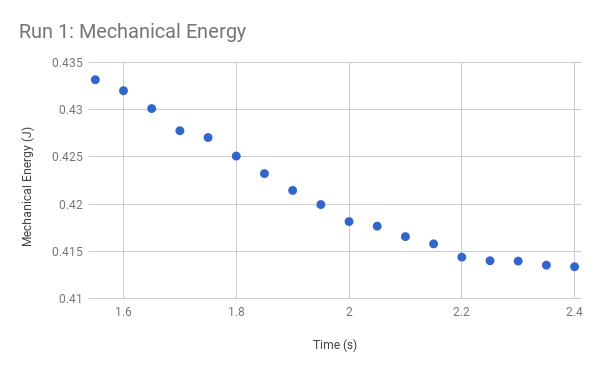
\includegraphics[scale=0.71]{image/07-mechanic/run-1-energy.png}
    \caption{}
    \label{figure.07.run.1.e}
\end{figure}
%%%%%%%%%%%%%%%%%%%%%%%%%%%%%%%%%%%%%%%%%%%%%%%%%%%%%%%%%%%%%%%%%%%%%%%%%%%%%%%%
\begin{figure}
    \centering
    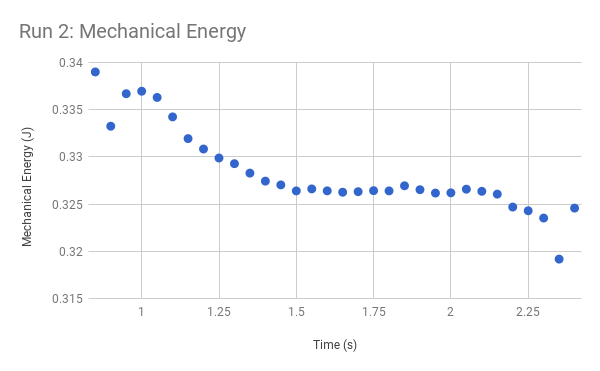
\includegraphics[scale=0.71]{image/07-mechanic/run-2-energy.png}
    \caption{}
    \label{figure.07.run.2.e}
\end{figure}
%%%%%%%%%%%%%%%%%%%%%%%%%%%%%%%%%%%%%%%%%%%%%%%%%%%%%%%%%%%%%%%%%%%%%%%%%%%%%%%%
\begin{figure}
    \centering
    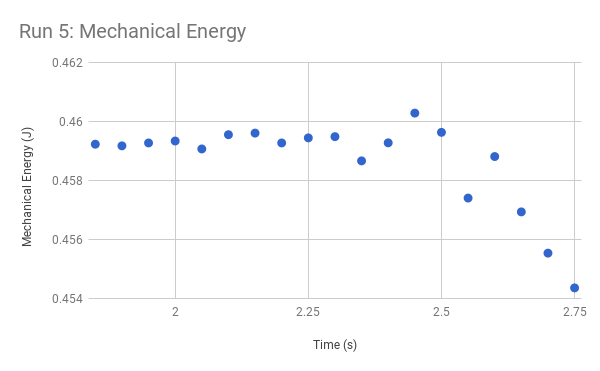
\includegraphics[scale=0.71]{image/07-mechanic/run-5-energy.png}
    \caption{}
    \label{figure.07.run.5.e}
\end{figure}
%%%%%%%%%%%%%%%%%%%%%%%%%%%%%%%%%%%%%%%%%%%%%%%%%%%%%%%%%%%%%%%%%%%%%%%%%%%%%%%%
\begin{figure}
    \centering
    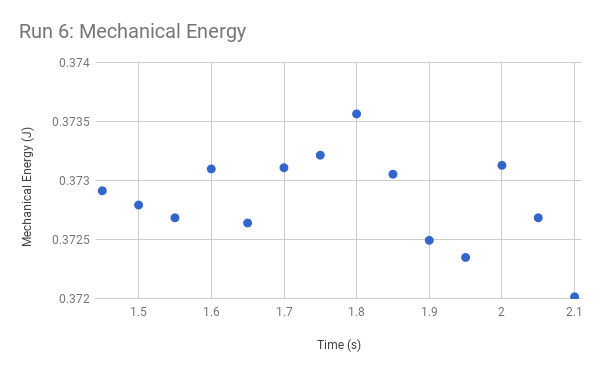
\includegraphics[scale=0.71]{image/07-mechanic/run-6-energy.png}
    \caption{}
    \label{figure.07.run.6.e}
\end{figure}
%%%%%%%%%%%%%%%%%%%%%%%%%%%%%%%%%%%%%%%%%%%%%%%%%%%%%%%%%%%%%%%%%%%%%%%%%%%%%%%%
\subsection{Calculate Velocity Squared}
%%%%%%%%%%%%%%%%%%%%%%%%%%%%%%%%%%%%%%%%%%%%%%%%%%%%%%%%%%%%%%%%%%%%%%%%%%%%%%%%
In a separate column, you should calculate the velocity squared using the values in the velocity column. If $v$ is a velocity values, then the velocity square is $v^2$ or equivalently $v \times v$.
%%%%%%%%%%%%%%%%%%%%%%%%%%%%%%%%%%%%%%%%%%%%%%%%%%%%%%%%%%%%%%%%%%%%%%%%%%%%%%%%
\subsection{Graph $v^2$ vs $h$}
%%%%%%%%%%%%%%%%%%%%%%%%%%%%%%%%%%%%%%%%%%%%%%%%%%%%%%%%%%%%%%%%%%%%%%%%%%%%%%%%
The other goal of this experiment was to verify the linear relation between $v^{2}$ and $h$ suggested by equation (\ref{eq.07.vv}) due to conservation of energy. Since the relation is a linear function, the data points should arrange themselves to form a linear shape. You can use Google Sheets or Excel to find the best linear fit. In Google Sheets, this is under ``Series'' in the chart editor. You need to check the ``Trend line'' box and make sure that it is ``Linear''. It is good practice to reduce the size of the data points (I use 2px) and to use a color for the trend line that is different from the color of the data points. In my case I have blue data points for the experimental data and red line for the best fit line.

If the data were perfect, then the slope of this linear fit should be given by
\begin{equation} \label{eq.07.slope}
    \text{slope } = -2g = 19.6 \text{ m/s}^{2}
\end{equation}
and the intercept would be related to the amount of mechanic energy via
\begin{equation}
    \text{intercept } = \frac{2 E}{m}
\end{equation}
The slope is negative, so we should see a diagonal line that is downward as height increases. From the intercept you can get a value for mechanic energy that should be close to what you found in the mechanic energy column:
\begin{equation} \label{eq.07.intercept}
    E = \frac{m \times \text{ intercept}}{2}
\end{equation}
You can also compare this value with the average of the mechanic energy column (use the \texttt{AVERAGE} function to compute this). Note that this is an average over time.
%%%%%%%%%%%%%%%%%%%%%%%%%%%%%%%%%%%%%%%%%%%%%%%%%%%%%%%%%%%%%%%%%%%%%%%%%%%%%%%%
\begin{figure}
    \centering
    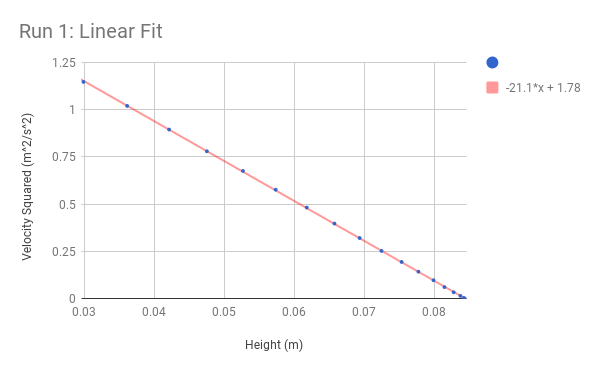
\includegraphics[scale=0.71]{image/07-mechanic/run-1-fit.png}
    \caption{}
    \label{figure.07.run.1.fit}
\end{figure}
%%%%%%%%%%%%%%%%%%%%%%%%%%%%%%%%%%%%%%%%%%%%%%%%%%%%%%%%%%%%%%%%%%%%%%%%%%%%%%%%
\begin{figure}
    \centering
    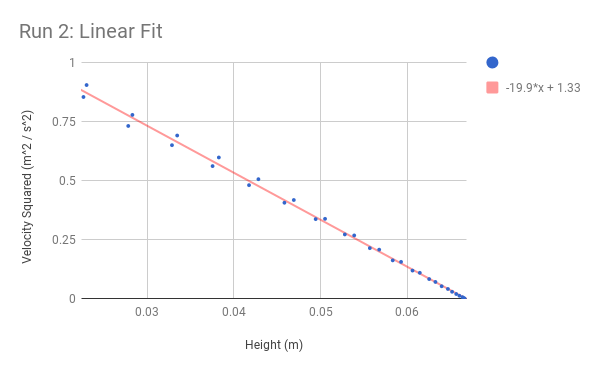
\includegraphics[scale=0.71]{image/07-mechanic/run-2-fit.png}
    \caption{}
    \label{figure.07.run.2.fit}
\end{figure}
%%%%%%%%%%%%%%%%%%%%%%%%%%%%%%%%%%%%%%%%%%%%%%%%%%%%%%%%%%%%%%%%%%%%%%%%%%%%%%%%
\begin{figure}
    \centering
    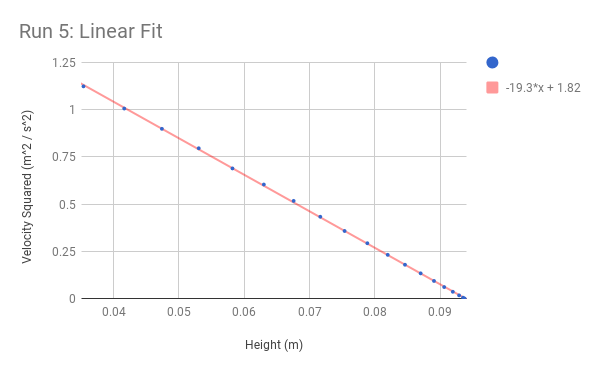
\includegraphics[scale=0.71]{image/07-mechanic/run-5-fit.png}
    \caption{}
    \label{figure.07.run.5.fit}
\end{figure}
%%%%%%%%%%%%%%%%%%%%%%%%%%%%%%%%%%%%%%%%%%%%%%%%%%%%%%%%%%%%%%%%%%%%%%%%%%%%%%%%
\begin{figure}
    \centering
    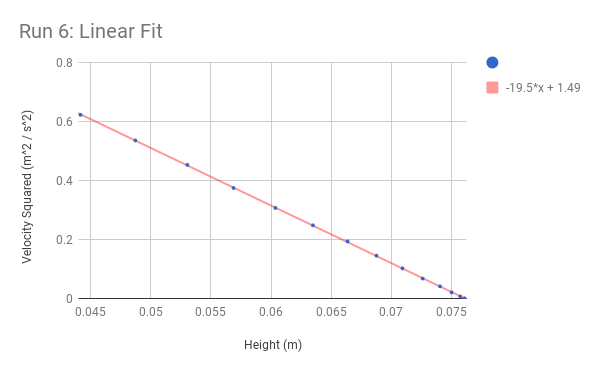
\includegraphics[scale=0.71]{image/07-mechanic/run-6-fit.png}
    \caption{}
    \label{figure.07.run.6.fit}
\end{figure}
%%%%%%%%%%%%%%%%%%%%%%%%%%%%%%%%%%%%%%%%%%%%%%%%%%%%%%%%%%%%%%%%%%%%%%%%%%%%%%%%
\section{My Data}
%%%%%%%%%%%%%%%%%%%%%%%%%%%%%%%%%%%%%%%%%%%%%%%%%%%%%%%%%%%%%%%%%%%%%%%%%%%%%%%%
I collected ten runs of data. In run 1, I used a truncation that only kept the upward motion. In run 2, I used a truncation that kept the upward and the downward motion. For run 5 and 6, I used a truncation that only kept the downward motion. As you can see, the linear fits are very appropriate, so the data does satisfy a linear relation. Furthermore, the values for the slope agree with the prediction: they are all very close to the predicted value in (\ref{eq.07.slope}). Also, the value of the intercept can be used in equation (\ref{eq.07.intercept}) to obtain an energy value that agrees with the time average mechanic energy.

Let us extract these values from a graph. Look at graph \ref{figure.07.run.6.fit} for run 6. The slope is -19.5 m/s$^{2}$. The intercept is 1.49 m$^{2}$/s$^{2}$. If the mass is 0.5 kg, then
\begin{equation}
    \frac{m \times \text{ intercept}}{2} = \frac{1}{2} (0.5 \text{ kg}) (1.49 \text{ m}^{2}\text{/s}^{2}) = 0.3717 \text{ J}
\end{equation}
This number is close to the time-average of the mechanic energy: 0.3728 J.

Here is a table summarizing some of my results.
%%%%%%%%%%%%%%%%%%%%%%%%%%%%%%%%%%%%%%%%%%%%%%%%%%%%%%%%%%%%%%%%%%%%%%%%%%%%%%%%
\begin{table}
	\centering
    \begin{tabular}{|r|r|r|r|r|}\hline
        Run & 1 & 2 & 5 & 6 \\ \hline
        Slope (m/s$^{2}$) & -21.1 & -19.9 & -19.3 & -19.5 \\
        Intercept (m$^{2}$/s$^{2}$) & 1.78 & 1.33 & 1.82 & 1.49 \\
        $E$ from intercept (J) & 0.4460 & 0.3326 & 0.4540 & 0.3717 \\
        Time-averaged $E$ (J) & 0.4210 & 0.3283 & 0.4587 & 0.3728 \\
        \hline
    \end{tabular}
    \caption{Summary of results}
    \label{table.07.results}
\end{table}
%%%%%%%%%%%%%%%%%%%%%%%%%%%%%%%%%%%%%%%%%%%%%%%%%%%%%%%%%%%%%%%%%%%%%%%%%%%%%%%%
\section{Your Data}
%%%%%%%%%%%%%%%%%%%%%%%%%%%%%%%%%%%%%%%%%%%%%%%%%%%%%%%%%%%%%%%%%%%%%%%%%%%%%%%%
You should have ten runs of data as well.
%%%%%%%%%%%%%%%%%%%%%%%%%%%%%%%%%%%%%%%%%%%%%%%%%%%%%%%%%%%%%%%%%%%%%%%%%%%%%%%%
\section{Your Laboratory Report}
%%%%%%%%%%%%%%%%%%%%%%%%%%%%%%%%%%%%%%%%%%%%%%%%%%%%%%%%%%%%%%%%%%%%%%%%%%%%%%%%
For your lab report, I want you to look at three of your ten runs. You are free to choose which three runs. For the first run you should use a truncation that leaves the upward motion only. For the second run, use a truncation with the downward motion only. For the third run, use a truncation with both upward and downward motion.

For each of the three runs you should
\begin{enumerate}
    \item produce a mechanic energy versus time graph
    \item produce a $v^{2}$ versus $h$ graph; include the best linear fit and extract the slope and the intercept
\end{enumerate}
You should also have a table like the one above summarizing the results (my table has four runs; your table should have three).